\section{Model of open-loop}
The feedback loop for controlling the output voltage will only consider perbutations to the duty cycle and its effect on the output voltage. In the small signal model from previous work the the input voltage will be considered as constant resulting in the simplified expressions of $G_{vc}$ from the lectures. The same expression for buck-boost converter is used, but with $D'$ replaced by $D'/n$ and the sign flipped, as the flyback converter inverts the output voltage compared to the buck-boost.

The transfer function from controller to output for the converter is thus
\[
G_{vc}(s) = R\cdot \frac{\frac{D'}{n}}{1+D}\cdot\frac{1-s\cdot \frac{D\cdot L}{(\frac{D'}{n})^2 \cdot R}}{1+s\cdot \frac{R\cdot C}{1+D}}
\]
With our values this becomes
\[
G_{vc}(s)=\frac{-0.057997\cdot (s - 6.028\cdot 10^4)}{s+2107}
\]
\begin{figure}[H]
    \centering
    \BodeZPK [blue,thick]
    {z/{6.0280e4},p/{-2107},k/-0.057997}
    {10}{10000000}
    \caption{bode plot of the controller-output transfer function}
    \label{fig:bp1}
\end{figure}
%i dont know how to do this :(

The gain margin is 24.7dB, with a phase margin of 124\degree at 444Hz.

\section{Type 2 Compensator}
We will be using the TL431 as a type 2 compensator
\subsection{Calculate R1 and Rb}
Since we will be using the TL431 as the current mode controller, the reference voltage is fixed at 2.5V. from this we can set the value of $R_1$ to be 10k$\Omega$, now the value of $R_b$ can be calculated from the voltage divider equation:
\[
\frac{V_o}{R_1 + R_b} \cdot R_b = V_{ref}
\]
as
\[
R_b = \frac{V_{ref}\cdot R_1}{V_o - V_{ref}} = 2k\Omega
\]
Thus: $R_1 = 10k\Omega$ and $R_b = 2k\Omega$
%\subsection{Loop gain phase bode plot}

\subsection{Cross over frequency}
The crossover frequency is chossen to be 5000Hz, at atteniuation of 18dB. This gives us a kp of $10^{\frac{18}{20}}=7.99$
\subsection{R4 and R5}
R5 is then found by:
\[
R5= \frac{V_o - V_f - V{k,min}}{I_k}
\]
Here $V_f$, $V_{k,min}$ and $I_k$ are given by the TL431, so R5 becomes:
\[
R5 = \frac{15V - 1.05V - 2.5V}{0.002A} = 5.725 k\Omega
\]
Then R4 can be found via the following with CTR being 1 at our operation point:% TODO find arguments that this is in fact our operation point
\[
R4 = \frac{kp \cdot R5}{CTR} = 45.726k\Omega
\]
\subsection{C1}
C1 is found via:
\[
C1=\frac{1}{2\cdot\pi\cdot f_z \cdot R1}
\]
$f_z$ is set to be $\frac{1}{5}$ of the crossover frequency, this in turn gives us a value for C1:
\[
C1 = \frac{1}{2\cdot\pi\cdot \frac{f_c}{5} \cdot 10k\Omega} = 3.1831 nF
\]
\subsection{C3}
C3 is like wise found by:
\[
C3 = \frac{1}{2\cdot\pi\cdot f_p \cdot R4}
\]
where $f_p$ is set to be 7 times higher than the crossover frequency, so:
\[
C3 = \frac{1}{2\cdot\pi\cdot (7f_c) \cdot 5.692k\Omega}=99.4 pF
\]
Initially $f_p$ was set 5 times higher than the crossover frequency, however to increase the gain margin the pole had to be pushed to a higher frequency.

\subsection{Verify frequency response}
The transfer function with the controller then becomes:
\[
H(s)=\frac{1.7565\cdot10^6(s + 6283)}{s(s+2.199\cdot10^5)}
\]
\begin{figure}[H]
    \centering
    \BodeZPK [blue,thick]
    {z/{-6283},p/{0,-2.99e5},k/1.7565e6}
    {10}{10000000}
    \caption{frequency response of the controller}
    \label{fig:bp2}
\end{figure}
\subsection{Verify loop stability}

\begin{figure}[H]
    \centering
    \BodeZPK [blue,thick]
    {z/{-6283,6.0280e4},p/{0,-2.99e5,-2107},k/-1.0187e5}
    {10}{10000000}
    \caption{Loop gain with controller ($G_{vc}(s)H(s)$)}
    \label{fig:bp3}
\end{figure}

The full loop has a gain margin of 6.5dB at 1.75kHz and a phase margin of 46.6\degree at the expected 5kHz.

\subsection{Circuit diagram}
\begin{figure}[H]
    \centering
    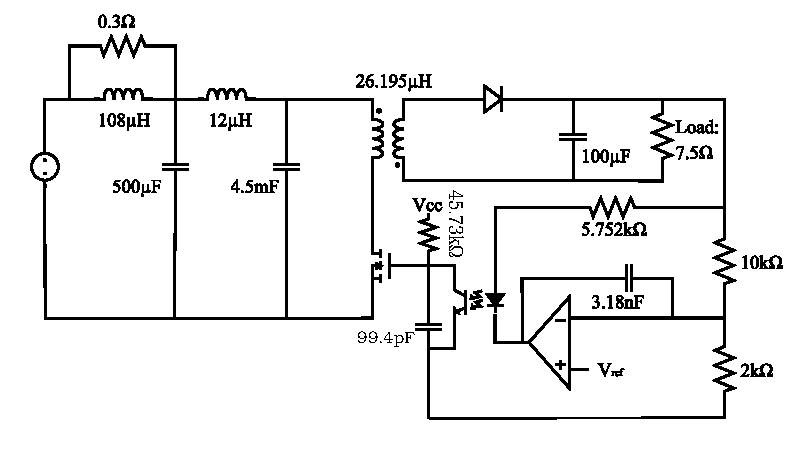
\includegraphics[width=\linewidth]{report_final/Pictures/schematic.pdf}
    \caption{Schematic of flyback converter with input filter, output filter and controller.}
    \label{fig:sch}
\end{figure}